\chapter{تصویر کلی علوم زبان و آواشناسی تولیدی}
\emergencystretch=4em
\newcommand{\chtwoFz}{F_{\text{\lr{0}}}}
\newcommand{\chtwoTz}{T_{\text{\lr{0}}}}

\section{مرور جلسهٔ قبل و تغییر رویکرد}

در جلسهٔ نخست مسئلهٔ پردازش زبان و گفتار را با رویکرد \term{بالا‌به‌پایین}{Top-Down} بررسی کردیم: ابتدا تسک‌های اصلی زبان (مانند \eng{POS Tagging}، \eng{NER}، \eng{Intent Detection}، \eng{Slot Filling}، \eng{Language Modeling} و \eng{Coreference Resolution}) و گفتار (مانند \eng{STT}، \eng{TTS}، \eng{Voice Activation}، \eng{Speaker Recognition} و \eng{Speaker Diarization}) معرفی شدند و سپس دیدیم که چگونه این تسک‌ها در یک \eng{Pipeline} کنار هم قرار می‌گیرند و محصولاتی مانند خلاصه‌ساز جلسات یا سامانهٔ احراز هویت آنلاین می‌سازند. در آن جلسه هنوز وارد جزئیات داده و مدل‌ها نشدیم.

از این جلسه مسیر را برعکس می‌کنیم و رویکرد \term{پایین‌به‌بالا}{Bottom-Up} را در پیش می‌گیریم:
\begin{enumerate}
  \item ابتدا خود \textbf{داده} را بشناسیم: داده‌ای که می‌خواهیم پردازش کنیم از چه جنسی است و چگونه به وجود می‌آید؟
  \item سپس به مفهوم \term{بازنمایی}{Representation} برسیم: چگونه داده را به شکلی درآوریم که کامپیوتر بتواند پردازش کند؟ این بازنمایی‌ها می‌توانند \textbf{دست‌ساز} (\eng{Handcrafted})، \textbf{یادگرفته‌شده} (\eng{Learned}) یا \textbf{یادگرفته‌شده با خودنظارتی} (\eng{Self-Supervised} \eng{Learned}) باشند.
  \item در پایان، با داشتن داده و بازنمایی مناسب، به سراغ مدل‌های پیچیده‌تر و عمیق‌تر برویم.
\end{enumerate}

\subsection{گفتار و متن: دو جنس متفاوت از داده}
نکتهٔ کلیدی این است که جنس دادهٔ گفتاری و متنی یکسان نیست. متن دنباله‌ای از نمادهاست، اما گفتار یک پدیدهٔ فیزیکی است که در هوا منتشر می‌شود.

\begin{table}[htbp]
\centering
\caption{مقایسهٔ ماهیت داده در متن و گفتار}
\begin{tabular}{p{0.38\textwidth} p{0.38\textwidth}}
\toprule
\textbf{گفتار} (\eng{Speech}) & \textbf{متن} (\eng{Text}) \\
\midrule
ماهیت فیزیکی دارد & ماهیت نمادین دارد \\
به‌صورت موج صوتی منتقل می‌شود & از نمادها و نشانه‌ها تشکیل شده است \\
در زمان پیوسته است & در سطح توالی نمادها گسسته است \\
\bottomrule
\end{tabular}
\end{table}

بر همین اساس، دو مسیر پردازش موازی داریم (شکل \ref{fig:ch02-pipelines}). در مسیر متن، زبان ابتدا به متن (دنبالهٔ نمادهای گسسته) تبدیل می‌شود، سپس بازنمایی زبانی از آن ساخته می‌شود و در نهایت تسک‌های \eng{NLP} روی آن اجرا می‌گردند. در مسیر گفتار، موج صوتی ابتدا به‌شکل سیگنال دیجیتال درمی‌آید، سپس بازنمایی آکوستیکی یا زبانی از آن استخراج می‌شود و در نهایت تسک‌های گفتاری انجام می‌شوند.

\begin{figure}[htbp]
\centering
\begin{tikzpicture}[rtl, 
  rtl,
  node distance=6mm,
  box/.style={draw, rounded corners, align=center, minimum height=1.05cm, text width=2.35cm, font=\footnotesize, fill=softblue},
  sbox/.style={box, fill=softyellow},
  arr/.style={-{Stealth[length=2.2mm]}, thick}]
\node[box] (l) {زبان};
\node[box, left=of l] (t) {متن\\ \lr{(Discrete / Symbolic)}};
\node[box, left=of t] (lr) {بازنمایی زبانی\\ \lr{Linguistic Rep.}};
\node[box, left=of lr] (nlp) {تسک‌های \lr{NLP}};
\draw[arr] (l) -- (t); \draw[arr] (t) -- (lr); \draw[arr] (lr) -- (nlp);
\node[sbox, below=7mm of l] (s) {گفتار};
\node[sbox, left=of s] (sg) {سیگنال\\ \lr{(Continuous / Physical)}};
\node[sbox, left=of sg] (ar) {بازنمایی آکوستیکی/زبانی};
\node[sbox, left=of ar] (st) {تسک‌های گفتاری};
\draw[arr] (s) -- (sg); \draw[arr] (sg) -- (ar); \draw[arr] (ar) -- (st);
\end{tikzpicture}
\caption{دو مسیر موازی پردازش زبان: متن (گسسته و نمادین) و گفتار (پیوسته و فیزیکی). بازترسیم نمودار تخته (شکل افزوده)}
\label{fig:ch02-pipelines}
\end{figure}

بنابراین در این جلسه ابتدا روی ماهیت داده گفتاری تمرکز می‌کنیم: موج صوتی چیست، چگونه ایجاد می‌شود و انسان چگونه صحبت می‌کند. پس از شناخت داده، گام بعدی (جلسات بعد) تبدیل آن به بازنمایی مناسب پردازش رایانه‌ای است.

\section{تصویر کلی: جایگاه پردازش گفتار در علوم زبان}

برای اینکه بدانیم این درس در کجای نقشهٔ علم قرار می‌گیرد، باید جایگاه \term{زبان‌شناسی}{Linguistics} را ببینیم. زبان‌شناسی در کنار علومی مانند فیزیک، ریاضی، روان‌شناسی و جامعه‌شناسی یکی از علوم مرتبط با موضوع ماست و خود شاخه‌های متعددی دارد (شکل \ref{fig:ch02-linguistics-map}).

\begin{figure}[htbp]
\centering
\resizebox{0.95\textwidth}{!}{%
\begin{tikzpicture}[rtl, font=\small, >=Stealth,
  inter/.style={draw=black!70, thick, rounded corners=4pt, minimum width=4cm, minimum height=1.3cm, align=center, fill=white},
  branch/.style={draw=black!70, thick, ellipse, minimum width=3.6cm, minimum height=1.5cm, align=center, fill=softyellow},
  note/.style={font=\footnotesize, align=center, text width=4.2cm, text=black!75},
  arr/.style={->, thick, black!75}]
\node[draw=black!70, thick, diamond, aspect=2.6, fill=softred, inner sep=2pt, minimum width=4.2cm] (L) at (0,0) {\lr{Linguistics}};
% interdisciplinary (top)
\node[inter, fill=softyellow] (CL) at (-6.2,2.6) {\lr{Computational}\\\lr{Linguistics}};
\node[note, above=1mm of CL] {مطالعهٔ مدل‌هایی که زبان را می‌فهمند};
\node[inter] (NL) at (0,3.2) {\lr{Neurolinguistics}};
\node[note, above=1mm of NL] {مطالعهٔ مکانیزم‌های عصبی مغز که مسئول پردازش زبان هستند};
\node[inter] (X1) at (6.2,2.6) {\ldots};
% branches (bottom)
\node[branch] (PH) at (-6.2,-3) {آواشناسی\\\lr{(Phonetics)}};
\node[branch] (SY) at (-2,-3.4) {نحو \lr{(Syntax)}};
\node[note, below=1mm of SY] {قواعد ترتیب کلمات برای ساخت جمله};
\node[branch] (MO) at (2.6,-3) {ریخت‌شناسی\\\lr{(Morphology)}};
\node[branch, minimum width=2.6cm] (X2) at (6.9,-3) {\ldots};
\foreach \t in {CL,NL,X1,PH,SY,MO,X2} \draw[arr] (L) -- (\t);
\end{tikzpicture}}
\caption{نقشهٔ شاخه‌های زبان‌شناسی و علوم میان‌رشته‌ای مرتبط با آن. شاخه‌های درونی (بیضی‌ها) شامل آواشناسی، نحو و ریخت‌شناسی‌اند و علوم میان‌رشته‌ای (مستطیل‌ها) شامل زبان‌شناسی رایانشی و عصب‌زبان‌شناسی. (بازسازی‌شده از تختهٔ کلاس)}
\label{fig:ch02-linguistics-map}
\end{figure}

\subsection{شاخه‌های اصلی زبان‌شناسی}
\begin{description}
  \item[\term{آواشناسی}{Phonetics}] مطالعهٔ صداهای گفتاری انسان: چگونه تولید می‌شوند، چه ویژگی‌های فیزیکی دارند و چگونه شنیده می‌شوند. این شاخه محور اصلی این جلسه و جلسات بعدی است.
  \item[\term{نحو}{Syntax}] قواعد ترتیب و چینش کلمات برای ساختن جمله. در \eng{NLP} بسیار با آن سروکار داریم.
  \item[\term{ریخت‌شناسی یا صرف}{Morphology}] ساختار درونی کلمات و تغییر شکل آن‌ها. برای نمونه صرف فعل «رفتن» (رفتم، رفتی، رفت، رفتیم، \ldots) یا واژه‌سازی: «دانش» + «ـمند» $\leftarrow$ «دانشمند» که در آن افزودن پسوند واژهٔ تازه‌ای می‌سازد.
  \item[شاخه‌های دیگر] روی تخته با «\ldots» نشان داده شده‌اند؛ مثلاً معناشناسی و کاربردشناسی.
\end{description}

\begin{addedbox}{آواشناسی در برابر واج‌شناسی}
\term{آواشناسی}{Phonetics} خود صداها را به‌صورت فیزیکی (تولید، انتقال، ادراک) بررسی می‌کند، در حالی که \term{واج‌شناسی}{Phonology} به نظام صداها در یک زبان می‌پردازد: کدام صداها در آن زبان معنا را تغییر می‌دهند و صداها چگونه کنار هم می‌نشینند. در این جلسه بیشتر با آواشناسی کار داریم؛ اما مفهوم «واج» که در ادامه می‌آید، از واج‌شناسی آمده است.
\end{addedbox}

\subsection{علوم میان‌رشته‌ای}
\begin{description}
  \item[\term{زبان‌شناسی رایانشی}{Computational Linguistics}] در تقاطع زبان‌شناسی، علوم کامپیوتر و هوش مصنوعی قرار دارد و به مدل‌سازی محاسباتی زبان (مدل‌هایی که زبان را پردازش، «می‌فهمند» یا تولید می‌کنند) می‌پردازد. درس ما، \term{پردازش زبان گفتاری}{Spoken Language Processing}، در همین چارچوب قرار می‌گیرد.
  \item[\term{عصب‌زبان‌شناسی}{Neurolinguistics}] در تقاطع زبان‌شناسی و علوم اعصاب است و سازوکارهای عصبی مغز را که مسئول پردازش زبان‌اند مطالعه می‌کند.
\end{description}

\begin{exambox}{نگاه مهندسی به زبان‌شناسی}
هدف ما به‌عنوان مهندس هوش مصنوعی ارائهٔ نظریهٔ تازه در همهٔ شاخه‌های زبان‌شناسی نیست؛ مفاهیم و دسته‌بندی‌های موردنیاز را از این علوم می‌شناسیم و در ساخت مدل‌های محاسباتی از آن‌ها بهره می‌گیریم. (بخش‌های بعدی نشان می‌دهد این دانش چگونه به کار می‌آید.)
\end{exambox}

\section{نظریهٔ زایشی چامسکی (۱۹۵۷)}

یکی از مباحث مهم در تاریخ زبان‌شناسی که ارتباط نزدیکی با علوم شناختی و هوش مصنوعی دارد، \term{نظریهٔ زایشی}{Generative Theory} نوآم چامسکی است. تخته این نظریه را با سال ۱۹۵۷ نشان داده است. (چامسکی در همان سال کتاب \eng{Syntactic Structures} را منتشر کرد.)

\begin{figure}[htbp]
\centering
\begin{tikzpicture}[rtl, font=\normalsize]
\node[draw=black!70, thick, rounded corners=5pt, inner sep=7pt, align=center, fill=boxgray] (t) at (0,0) {\textbf{نظریهٔ زایشی چامسکی}\\\textbf{۱۹۵۷}};
\node[text width=0.88\textwidth, align=center, below=5mm of t] (a) {دیدگاه اولیه: یادگیری زبان از طریق تقلید و تکرار\\
رد این دیدگاه با نظریهٔ زایشی: جملات جدیدی که کودک می‌سازد؛ پس درون ذهن انسان مکانیسم‌هایی وجود دارد (کمک به شکل‌گیری علوم شناختی)};
\node[text width=0.88\textwidth, align=center, below=4mm of a, text=green!45!black] (b) {\textbf{زبان خطی نیست، بلکه سلسله‌مراتبی و درختی است}};
\node[text width=0.88\textwidth, align=center, below=4mm of b, text=red!65!black] (c) {انسان از بدو تولد قواعد زبانی جهان‌شمول \lr{\mbox{Universal Grammar}} دارد و بعد از تولد، طبق محیط، پارامترها را تنظیم می‌کند.\\
یادگیری زبان به صورت آماری و توزیعی است: با قرارگیری در محیط و دیدن نمونه‌های زیاد، قواعد را یاد می‌گیرد.};
\end{tikzpicture}
\caption{خلاصهٔ نظریهٔ زایشی چامسکی: رد دیدگاه تقلیدی (سیاه)، ساختار سلسله‌مراتبی و درختی زبان (سبز) و دو دیدگاه دربارهٔ منشأ قواعد زبان (قرمز): دستور جهانی با تنظیم پارامترها، در برابر یادگیری آماری و توزیعی. (بازسازی‌شده از تختهٔ کلاس)}
\end{figure}

\subsection{دیدگاه تقلیدی و نقد آن}
در دیدگاه قدیمی‌تر، یادگیری زبان عمدتاً حاصل \textbf{تقلید و تکرار} دانسته می‌شد: کودک جمله‌ای را از اطرافیان می‌شنود، حفظ می‌کند و در موقعیت مشابه آن را تکرار می‌کند. چامسکی این نگاه را با این استدلال رد کرد که کودکان به‌طور مرتب \textbf{جمله‌های جدیدی} می‌سازند که هرگز نشنیده‌اند؛ حتی کلمه‌های تازه می‌سازند یا کلمات را در ساختارهایی به کار می‌برند که پیش‌تر آن ترکیب را ندیده‌اند. پس توانایی زبانی چیزی بیش از حفظ جمله‌هاست و باید در ذهن انسان سازوکارهایی وجود داشته باشد که جمله‌های تازه را «تولید» (\eng{generate}) کند. همین ایده بعدها به شکل‌گیری علوم شناختی کمک کرد.

\subsection{زبان خطی نیست، سلسله‌مراتبی است}
بر اساس این نظریه، جمله فقط دنبالهٔ خطی کلمات نیست، بلکه ساختاری \term{سلسله‌مراتبی}{Hierarchical} و درختی دارد (شکل \ref{fig:ch02-tree}). کلمات به گروه‌هایی (مانند گروه اسمی و گروه فعلی) سازمان می‌یابند و گروه‌ها در هم تو در تو می‌شوند.

\begin{figure}[htbp]
\centering
\begin{tikzpicture}[rtl, 
  level distance=11mm,
  every node/.style={font=\small},
  cat/.style={font=\small\itshape}]
\node (S) at (0,0) {\lr{S}};
\node (NP1) at (1.8,-1.2) {\lr{NP}};
\node (VP) at (-1.8,-1.2) {\lr{VP}};
\node (N1) at (1.8,-2.4) {\lr{N}};
\node (w1) at (1.8,-3.4) {کودک};
\node (NP2) at (0,-2.4) {\lr{NP}};
\node (V) at (-3,-2.4) {\lr{V}};
\node (w3) at (-3,-3.4) {خورد};
\node (N2) at (0.8,-3.4) {\lr{N}};
\node (P) at (-0.8,-3.4) {\lr{P}};
\node (w2) at (0.8,-4.4) {سیب};
\node (w2b) at (-0.8,-4.4) {را};
\draw (S)--(NP1); \draw (S)--(VP);
\draw (NP1)--(N1); \draw (N1)--(w1);
\draw (VP)--(NP2); \draw (VP)--(V); \draw (V)--(w3);
\draw (NP2)--(N2); \draw (NP2)--(P); \draw (N2)--(w2); \draw (P)--(w2b);
\end{tikzpicture}
\caption{نمونهٔ ساده‌شدهٔ درخت ساختار سلسله‌مراتبی برای جملهٔ «کودک سیب را خورد». \lr{S}: جمله، \lr{NP}: گروه اسمی، \lr{VP}: گروه فعلی، \lr{N}: اسم، \lr{V}: فعل، \lr{P}: حرف اضافه (نشانهٔ «را»). (شکل افزوده)}
\label{fig:ch02-tree}
\end{figure}

\begin{addedbox}{چرا ساختار درختی لازم است؟ دو مثال}
\begin{itemize}
  \item \textbf{ابهام ساختاری:} جملهٔ «مرد دختر را با دوربین دید» دو معنی دارد (دوربین در دست مرد است یا دختر دوربین دارد). کلمات یکی‌اند؛ تنها درخت تحلیل متفاوت است. دنبالهٔ خطی کلمات برای تمایز این دو کافی نیست.
  \item \textbf{جملهٔ معروف چامسکی:} \eng{``Colorless green ideas sleep furiously''} از نظر دستوری درست اما بی‌معناست، و نشان می‌دهد درستیِ ساختار با احتمال کلمات یا معنا یکی نیست.
\end{itemize}
\end{addedbox}

\subsection{دستور جهانی در برابر یادگیری آماری}
پرسش اصلی این است: چه مقدار از توانایی زبانی از ابتدا در ذهن وجود دارد و چه مقدار از تجربه و داده یاد گرفته می‌شود؟ دو دیدگاه روی تخته آمده است:
\begin{enumerate}
  \item \textbf{دستور جهانی} (\term{دستور جهانی}{Universal Grammar}): انسان از بدو تولد صاحب اصول و قواعد زبانیِ جهان‌شمول است و پس از تولد، متناسب با محیط زبانی خود «پارامترها» را تنظیم می‌کند. کودکی که در محیط فارسی‌زبان رشد می‌کند فارسی و کودک انگلیسی‌زبان، انگلیسی را فرا می‌گیرد. (در کلاس این ایده با تنظیم پارامترهای یک مدل مقایسه شد: ساختار اولیه وجود دارد و تجربهٔ محیطی شکل نهایی عملکرد آن را تعیین می‌کند.)
  \item \textbf{یادگیری آماری و توزیعی} (\term{یادگیری توزیعی}{Distributional / Statistical Learning}): یادگیری زبان آماری است؛ انسان با قرارگرفتن در محیط و دیدن نمونه‌های بسیار، قواعد را از الگوهای آماری داده یاد می‌گیرد.
\end{enumerate}

برای پرسش «اگر کودک از ابتدا ساختاری دارد، دقیقاً چه چیزی را می‌داند و چه چیزی را یاد می‌گیرد؟» مقایسه با یادگیری عمیق مفید است: در یک شبکهٔ عصبی، معماری از پیش تعیین شده، اما الگوها و روابط را از داده می‌آموزد. می‌توان پرسید آیا در انسان هم ساختار عصبی اولیه وجود دارد ولی قواعد خاص هر زبان از تجربه فرا گرفته می‌شود؟ نقدهایی که به تفسیر سخت‌گیرانهٔ دستور جهانی وارد می‌شود عبارت‌اند از:
\begin{itemize}
  \item تفاوت‌های ساختاری میان زبان‌های مختلف؛
  \item شواهد یادگیری الگوهای جدید صرفاً از مواجهه با داده؛
  \item ابهام دربارهٔ اینکه دقیقاً کدام ویژگی‌های زبانی فطری‌اند.
\end{itemize}

جمع‌بندی کلاس: ایدهٔ زایشی و سلسله‌مراتبی‌بودن زبان همچنان اهمیت دارد، اما ادعای وجود مجموعه‌ای مشخص از قواعد دستوری مادرزادی محل بحث و نقد است. میزان فطری‌بودن زبان همچنان موضوعی پژوهشی و مورد اختلاف است.

\begin{correctionbox}{دقت تاریخی و فنی دربارهٔ نظریهٔ چامسکی}
\begin{itemize}
  \item سال ۱۹۵۷ سال انتشار \eng{Syntactic Structures} است که نحو صوری و زایشی را بنیان نهاد؛ هستهٔ استدلال علیه رویکرد «تقلیدی/رفتارگرا» (نقد چامسکی بر کتاب \eng{Verbal Behavior} اسکینر) در سال ۱۹۵۹ منتشر شد. صورت‌بندی «اصول و پارامترها» که در تخته آمده، بعدتر (دههٔ ۱۹۸۰) پدید آمد؛ بنابراین بهتر است آن را بخشی از تحول بعدی نظریه بدانیم، نه محتوای دقیق مقالهٔ ۱۹۵۷.
  \item استدلال اصلی به نفع ساختار فطری معمولاً «فقر محرک» (\eng{Poverty of the Stimulus}) خوانده می‌شود: داده‌ای که کودک می‌شنود برای تعیین یکتای قواعد کافی نیست. مخالفان (رویکردهای مبتنی بر کاربرد و یادگیری آماری) نشان می‌دهند کودکان و حتی نوزادان به الگوهای آماری گفتار حساس‌اند.
  \item دو دیدگاه الزاماً دو سر یک طیف‌اند، نه دو گزینهٔ کاملاً ناسازگار: بسیاری از پژوهشگران امروز بر ترکیبی از سوگیری‌های شناختی ذاتی و یادگیری از داده تأکید می‌کنند.
\end{itemize}
\end{correctionbox}

\begin{addedbox}{ارتباط با مدل‌های زبانی امروزی}
مدل‌های زبانی بزرگ، که تنها از توزیع آماری متن آموخته می‌شوند، در عمل تا حد زیادی ساختارهای نحوی را بازتولید می‌کنند. این موضوع به مناظرهٔ دستور جهانی در برابر یادگیری توزیعی دامن زده است؛ اما اینکه این مدل‌ها «شبیه کودک» یاد می‌گیرند یا نه، پرسشی باز است (مقدار داده‌ای که مدل‌ها می‌بینند چندین مرتبه بیشتر از داده‌ای است که کودک دریافت می‌کند).
\end{addedbox}

\section{ورود به آواشناسی}

\term{آواشناسی}{Phonetics} به مطالعهٔ صداهای گفتاری انسان می‌پردازد و دو بخش اصلی دارد:
\begin{description}
  \item[\term{آواشناسی تولیدی}{Articulatory Phonetics}] مطالعهٔ اینکه بدن انسان چگونه صدا می‌سازد؛ مثلاً برای تولید یک صدای مشخص، لب‌ها، زبان، فک و تارهای صوتی چه کاری انجام می‌دهند. موضوع این جلسه است.
  \item[\term{آواشناسی آکوستیکی}{Acoustic Phonetics}] بررسی خود موج صوتی و ویژگی‌های فیزیکی آن، بدون تمرکز بر اندام تولیدکننده. موضوع جلسهٔ بعد است.
\end{description}
هدف نهایی این است که پس از شناخت دادهٔ گفتاری، آن را به یک بازنمایی مناسب پردازش رایانه‌ای تبدیل کنیم.

\subsection{مثال آرتیکولاتور مکانیکی}
برای روشن‌شدن معنای واژهٔ \eng{articulation} از دستگاه \textbf{آرتیکولاتور مکانیکی} (\eng{Mechanical} \eng{Articulator}) که در دندان‌پزشکی استفاده می‌شود مثال زده شد: این دستگاه حرکات فک و تماس دندان‌ها را شبیه‌سازی می‌کند و قالب دندان بیمار روی آن قرار می‌گیرد تا ببینند هنگام حرکت فک چه اتفاقی می‌افتد. در گفتار نیز \textbf{آرتیکولیشن} یعنی نحوهٔ حرکت و هماهنگی اندام‌های گفتاری برای ساختن صداها.

\begin{correctionbox}{دقت در تشبیه}
این مثال فقط برای ایجاد شهود دربارهٔ واژهٔ \eng{articulate} (به‌معنای «مفصل‌بندی» و حرکت اجزای متصل به هم) است. در آواشناسی، \eng{articulators} به خود اندام‌های متحرک (لب‌ها، زبان، فک، نرم‌کام و \ldots) گفته می‌شود و ربطی به دستگاه دندان‌پزشکی ندارد.
\end{correctionbox}

\begin{figure}[htbp]
\centering
\begin{subfigure}[b]{0.3\textwidth}
\centering
\fbox{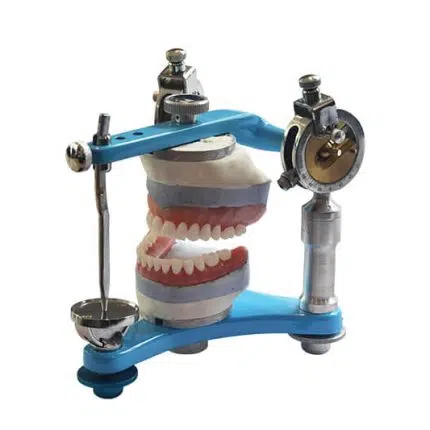
\includegraphics[width=0.94\textwidth]{../assets/figures/ch02-articulator.png}}
\caption{آرتیکولاتور مکانیکی}
\end{subfigure}\hfill
\begin{subfigure}[b]{0.62\textwidth}
\centering
\fbox{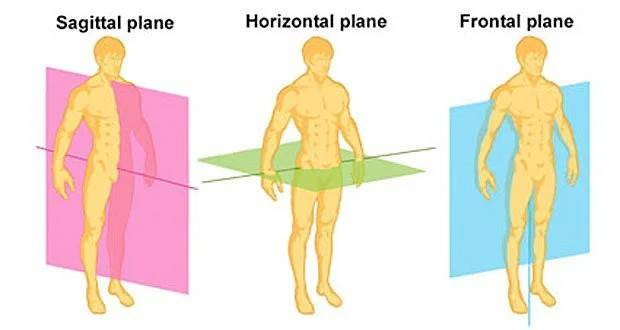
\includegraphics[width=0.97\textwidth]{../assets/figures/ch02-body-planes.png}}
\caption{صفحات حرکتی بدن}
\end{subfigure}
\caption{آرتیکولاتور مکانیکی دندان‌پزشکی و سه صفحهٔ مرجع آناتومی. \textit{(برگرفته از تختهٔ کلاس)}}
\label{fig:ch02-articulator-planes}
\end{figure}

\section{آناتومی تولید گفتار}

\subsection{صفحات آناتومیکی}
در آناتومی، بدن را با سه صفحهٔ مرجع از جهت‌های مختلف بررسی می‌کنند (شکل \ref{fig:ch02-articulator-planes}):
\begin{itemize}
  \item \term{صفحهٔ ساجیتال}{Sagittal}: بدن را به دو نیمهٔ چپ و راست تقسیم می‌کند (نمای از پهلو)؛
  \item \term{صفحهٔ فرونتال (پیشانی)}{Frontal / Coronal}: بدن را به بخش جلویی و پشتی تقسیم می‌کند؛
  \item \term{صفحهٔ افقی}{Horizontal / Transverse}: بدن را به بخش بالایی و پایینی تقسیم می‌کند.
\end{itemize}
برای مطالعهٔ حنجره، نای، دهان و مسیر عبور هوا، \textbf{نمای ساجیتال} بیشترین کاربرد را دارد، چون همهٔ این اجزا از پهلو در یک برش دیده می‌شوند (شکل \ref{fig:ch02-sagittal}).

\boardfigure{0.62}{ch02-vocal-tract-sagittal.png}{برش ساجیتال مجرای صوتی: حفرهٔ بینی، حلق، تارهای صوتی (درون حنجره)، نای و ریه‌ها.}
\label{fig:ch02-sagittal}

\subsection{اندام‌های اصلی}
\begin{table}[htbp]
\centering
\caption{اندام‌های اصلی دخیل در تولید گفتار}
\small
\begin{tabular}{p{2.9cm} p{3.6cm} p{6.6cm}}
\toprule
\textbf{اندام} & \textbf{معادل انگلیسی} & \textbf{نقش} \\
\midrule
ریه‌ها & \eng{Lungs} & منبع جریان هوا (تأمین فشار) \\
دیافراگم & \eng{Diaphragm} & ماهیچهٔ اصلی دم؛ کمک به تنفس \\
نای & \eng{Trachea} & مسیر عبور هوا از ریه به حنجره \\
حنجره & \eng{Larynx} & محل قرارگیری تارهای صوتی \\
تارهای صوتی & \eng{Vocal Folds} & تولید صوت واک‌دار از راه ارتعاش \\
حلق & \eng{Pharynx} & بخشی از مجرای صوتی بالای حنجره \\
حفرهٔ بینی (پشت بینی) & \eng{Nasal Cavity} & مشارکت در تولید صداهای خیشومی \\
دهان، زبان، لب‌ها، فک، دندان‌ها & \eng{Oral Articulators} & شکل‌دهی و تمایز صداهای گفتاری \\
\bottomrule
\end{tabular}
\end{table}

روی تخته تأکید شد که تارهای صوتی \textbf{زیر حلق} و در ابتدای نای، درون حنجره قرار دارند.

\begin{addedbox}{سه زیرسامانهٔ تولید گفتار}
می‌توان اندام‌های بالا را در سه گروه دید: (۱) \textbf{سامانهٔ تنفسی} (ریه، دیافراگم، نای) که انرژی و فشار هوا را فراهم می‌کند؛ (۲) \textbf{حنجره} که با ارتعاش تارهای صوتی «منبع صدا» را می‌سازد؛ (۳) \textbf{مجرای صوتی} (حلق، دهان و بینی) که با شکل‌های مختلف خود صدای منبع را فیلتر و شکل‌دهی می‌کند. این تصویر ساده‌ترین شکل مدل «منبع–فیلتر» است که در جلسهٔ بعد، هنگام بررسی فرمنت‌ها، به آن برمی‌گردیم.
\end{addedbox}

\subsection{دم و بازدم و ارتباط آن با گفتار}
تنفس در اصل برای ادامهٔ حیات است: با دم، هوا به ریه‌ها وارد می‌شود تا اکسیژن لازم تأمین شود و با بازدم، دی‌اکسیدکربن خارج می‌گردد. اما انسان از همین سامانه برای ساخت گفتار هم استفاده می‌کند.
\begin{description}
  \item[دم (\eng{Inhalation})] دیافراگم منقبض می‌شود و به‌سمت پایین می‌رود. حجم قفسهٔ سینه زیاد و فشار درون ریه کم می‌شود و هوا به ریه می‌آید. تارهای صوتی در تنفس معمولی باز (از هم دور) هستند تا هوا با کم‌ترین مقاومت عبور کند.
  \item[بازدم (\eng{Exhalation})] دیافراگم به حالت استراحت برمی‌گردد و هوا از ریه‌ها خارج می‌شود. این جریان هوا را می‌توان به‌عنوان «منبع انرژی» برای گفتار به کار گرفت: در گفتار واک‌دار هوا هنگام عبور از حنجره تارهای صوتی را به ارتعاش درمی‌آورد و صدای حاصل در بخش‌های بالاتر مجرا شکل می‌گیرد. (در تخته: «دیافراگم در دم فعال است و در بازدم ریلکس.»)
\end{description}

\begin{correctionbox}{دقت دربارهٔ بازدم در هنگام گفتار}
«دیافراگم در بازدم ریلکس است» دربارهٔ تنفس آرام درست است، اما در \textbf{گفتار} بازدم کاملاً منفعل نیست. اگر ریه فقط به‌حال خود رها شود، فشار هوا هنگام پر بودن ریه زیاد و هنگام خالی‌شدن آن کم می‌شود. برای اینکه فشار زیر حنجره در طول جمله تقریباً ثابت بماند (حدود ۵ تا ۱۰ سانتی‌متر آب برای گفتار معمولی)، سامانهٔ عصبی–عضلانی دائماً مداخله می‌کند: در ابتدای جمله عضلات دمی بازدم را «ترمز» می‌کنند و در انتها عضلات بازدمی (مانند بین‌دنده‌ای‌های داخلی و شکمی) هوا را به بیرون می‌رانند. به همین دلیل مکث‌های گفتار معمولاً با دم‌های کوتاه و سریع و بازدم‌های بلند و کنترل‌شده همراه است.
\end{correctionbox}

\paragraph{پرسش کلاسی: اگر هوا هنگام دم هم از تارهای صوتی می‌گذرد، چرا معمولاً هنگام بازدم صحبت می‌کنیم؟}
جمع‌بندی بحث چنین است:
\begin{itemize}
  \item در دم آرام تارهای صوتی باز هستند و هوا بدون ارتعاش از بین آن‌ها می‌گذرد؛ برای تولید صدای واک‌دار باید تارها به هم نزدیک شوند و در معرض جریان هوا با فشار کافی قرار گیرند.
  \item گفتار هنگام دم غیرممکن نیست: برخی افراد (و در برخی آوازها و تمرین‌های صوتی) می‌توانند در دم هم صدا یا گفتار تولید کنند، و گاهی در گفتار محاوره‌ای برخی زبان‌ها واژه‌هایی کوتاه (مانند «بله») با هوای دمی ادا می‌شوند. اما الگوی غالب گفتار در همهٔ زبان‌ها استفاده از هوای بازدمی است.
\end{itemize}

\begin{addedbox}{چرا بازدم؟}
دلیل‌های عملی ترجیح بازدم عبارت‌اند از: (۱) در بازدم می‌توان فشار هوا را برای مدت طولانی و با دقت کنترل کرد، در حالی که دم باید کوتاه و سریع باشد تا گفتار قطع نشود؛ (۲) ریه‌ها به‌طور طبیعی با بازگشت ارتجاعی هوا را بیرون می‌دهند، پس منبع فشار آمادهٔ بازدم وجود دارد، ولی در دم باید با کار ماهیچه‌ای هوا را به درون کشید. صدای تولیدشده در دم معمولاً ضعیف‌تر و کم‌کنترل‌تر است. این‌ها توضیح‌های تکمیلی‌اند، نه تمام ماجرا.
\end{addedbox}

\subsection{نای: چرا حلقه‌حلقه است؟}
نای (\eng{Trachea}) لولهٔ حدود ۱۰ تا ۱۲ سانتی‌متری است که هوا را از حنجره به ریه‌ها می‌برد. دیوارهٔ آن \textbf{حلقه‌های غضروفی} (حدود ۱۶ تا ۲۰ حلقه‌ی \eng{C}-شکل) دارد. این ساختار دو نقش دارد:
\begin{enumerate}
  \item \textbf{باز نگه‌داشتن مجرا:} هنگام دم فشار درون نای کمتر از فشار بیرون آن می‌شود. اگر دیواره نرم و بدون ساختار نگه‌دارنده بود، مانند یک نی نرم که هنگام مکیدن پهن می‌شود، تحت اختلاف فشار روی هم می‌خوابید و مسیر هوا بسته می‌شد.
  \item \textbf{انعطاف‌پذیری:} با اینکه لوله باز نگه داشته می‌شود، فاصلهٔ میان حلقه‌ها به نای (و گردن) اجازهٔ خم‌شدن، کشیده‌شدن و حرکت می‌دهد.
\end{enumerate}
بنابراین نای باید \textbf{همیشه باز} بماند؛ برخلاف تارهای صوتی که قرار است مرتب باز و بسته شوند.

\begin{addedbox}{جزئیات تکمیلی دربارهٔ نای}
حلقه‌های غضروفی کامل نیستند و در دیوارهٔ پشتی که به مری چسبیده، به‌شکل «\eng{C}» باز می‌مانند و این بخش را یک ماهیچهٔ صاف و غشای نرم می‌پوشاند. این طراحی به مری اجازه می‌دهد هنگام بلع غذا کمی به‌سمت نای برآمده شود.
\end{addedbox}

\section{حنجره و تارهای صوتی}

هوای خروجی ریه‌ها هنگام بازدم به حنجره می‌رسد. در حنجره جفت \term{تار صوتی}{Vocal Folds} قرار دارد که می‌تواند به هم نزدیک یا از هم دور شود (شکل \ref{fig:ch02-larynx}). فضای میان دو تار \term{چاکنای}{Glottis} نام دارد. در تنفس آرام این فاصله باز است و هنگام تولید صدای واک‌دار تارها به هم نزدیک می‌شوند و وارد چرخهٔ ارتعاش می‌شوند.

\boardfigure{0.55}{ch02-larynx-endoscopy.png}{نمای افقی (از بالا) از حنجرهٔ سالم با دوربین درون‌بین. دو تار صوتی (راست و چپ) و فاصلهٔ باز میان آن‌ها (چاکنای) دیده می‌شود؛ درون فضای تیره حلقه‌های نای قابل مشاهده است.}
\label{fig:ch02-larynx}

\begin{correctionbox}{«تار» یا «چین»؟}
واژهٔ رایج «تارهای صوتی» ترجمهٔ تحت‌اللفظی \eng{vocal cords} است و تصویر نادرستی از رشته یا سیم کشیده‌شده می‌دهد. اصطلاح علمی امروزی \eng{vocal folds} (چین‌های صوتی) است: هر تار صوتی توده‌ای از بافت ماهیچه‌ای و مخاطی است که در دو طرف مجرای حنجره از جلو (غضروف تیروئید) تا پشت (غضروف‌های آریتنوئید) امتداد دارد و با چرخش غضروف‌های آریتنوئید به هم نزدیک یا از هم دور می‌شود. در این جزوه، به‌دلیل رواج، همان «تارهای صوتی» را به کار می‌بریم. طول تارها در مردان بزرگسال حدود ۱۷ تا ۲۵ و در زنان حدود ۱۲ تا ۱۷ میلی‌متر است.
\end{correctionbox}

\subsection{چرا تارها فقط یک بار باز نمی‌شوند؟ اصل برنولی}
\paragraph{پرسش:} وقتی هوا از ریه‌ها بیرون می‌آید و از میان تارها می‌گذرد، چرا تارها یک بار باز نمی‌شوند و همان‌طور باز نمی‌مانند؟ چرا مرتب باز و بسته می‌شوند؟

برای پاسخ، \term{اصل برنولی}{Bernoulli's Principle} مطرح شد: در یک سیال در حال جریان، هرجا سرعت زیادتر باشد، فشار (ایستا) کمتر است. روی تخته: «شاره‌ای که سریع‌تر حرکت می‌کند فشار کمتری خواهد داشت.»

\begin{definitionbox}{اصل برنولی}
برای جریان پایا، تراکم‌ناپذیر و بدون اصطکاک در امتداد یک خط جریان:
\[
p + \tfrac{1}{2}\rho v^2 + \rho g h = \text{ثابت}
\]
که $p$ فشار ایستا، $\rho$ چگالی سیال، $v$ سرعت و $h$ ارتفاع است. در ارتفاع ثابت، افزایش سرعت ($v$) به‌معنای کاهش فشار ایستا ($p$) است.
\end{definitionbox}

\paragraph{آزمایش دو بطری.} اگر دو بطری سبک (خالی) را نزدیک هم بگذاریم و میان آن‌ها هوا بدمیم، برخلاف انتظار اولیه، بطری‌ها از هم دور نمی‌شوند بلکه به هم نزدیک می‌شوند. دلیل این است که سرعت هوا در فاصلهٔ میان بطری‌ها زیاد می‌شود، فشار آن ناحیه از فشار محیط بیرون کمتر می‌شود و اختلاف فشار بطری‌ها را به هم نزدیک می‌کند.

\paragraph{ارتباط با تارهای صوتی.} روایت ساده‌شدهٔ کلاس از چرخهٔ ارتعاش:
\begin{enumerate}
  \item تارها نزدیک هم‌اند و مجرا بسته است؛ فشار هوای زیر تارها بالا می‌رود.
  \item فشار زیر حنجره از حدی بیشتر می‌شود و تارها را از هم باز می‌کند.
  \item هوا با سرعت زیاد از شکاف باریک میان تارها عبور می‌کند.
  \item طبق اصل برنولی فشار در شکاف کم می‌شود و همراه با نیروی ارتجاعی بافت، تارها دوباره به هم نزدیک می‌شوند و مجرا بسته می‌شود.
  \item چرخه تکرار می‌شود و ارتعاش دوره‌ای هوا موج صوتی می‌سازد.
\end{enumerate}
از آنجا که این حرکت تکرارشونده است، می‌توان برای آن \textbf{فرکانس} تعریف کرد؛ همان \term{فرکانس پایه}{Fundamental Frequency, F0} که به‌صورت زیر یا بم‌بودن صدا ادراک می‌شود.

\boardfigure{0.5}{ch02-vocal-fold-cycle.png}{ده برش پیشانی (کرونال) متوالی از حنجره در یک چرخهٔ ارتعاش، از بسته‌بودن کامل تارها تا باز‌شدن و دوباره بسته‌شدن. دیده می‌شود که لبهٔ پایینی تارها زودتر از لبهٔ بالایی از هم جدا و زودتر به هم نزدیک می‌شود.}
\label{fig:ch02-fold-cycle}

\begin{correctionbox}{اصل برنولی تنها توضیح ارتعاش نیست}
توضیح کلاس مدلی ساده‌شده بود. نظریهٔ پذیرفته‌شده برای تولید صدا \term{نظریهٔ ماهیچه‌ای–ارتجاعی–آیرودینامیکی}{Myoelastic-Aerodynamic Theory} است (ون دن‌برگ، ۱۹۵۸). بر اساس آن:
\begin{itemize}
  \item ماهیچه‌های حنجره تارها را به هم نزدیک و کشش لازم را فراهم می‌کنند (\emph{myo}). مادامی که تارها بسته‌اند، فشار زیر چاکنا بالا می‌رود.
  \item فشار زیرحنجره‌ای تارها را از هم باز می‌کند و هوا می‌گذرد (\emph{aerodynamic}).
  \item نیروی ارتجاعی (بازگشتی) بافت تارها و نیروی کاهش فشار ناشی از افزایش سرعت جریان (اثر برنولی) و نیز کاهش فشار پایین‌دست آن‌ها را دوباره می‌بندد (\emph{elastic}).
\end{itemize}
اثر برنولی تنها یکی از نیروهای دخیل است. برای تداوم ارتعاش هم لازم است در هر چرخه انرژی از جریان هوا به بافت منتقل شود؛ این کار با تفاوت فاز میان لبهٔ پایینی و بالایی تارها (شکل \ref{fig:ch02-fold-cycle}) و تغییر شکل شکاف از همگرا به واگرا انجام می‌شود.
\end{correctionbox}

\begin{figure}[htbp]
\centering
\begin{tikzpicture}[rtl, scale=1, rtl]
% pipe
\draw[thick] (0,1) -- (2,1) .. controls (3,1) and (3,0.35) .. (4,0.35) -- (6,0.35);
\draw[thick] (0,-1) -- (2,-1) .. controls (3,-1) and (3,-0.35) .. (4,-0.35) -- (6,-0.35);
\draw[-{Stealth}, thick, blue!60!black] (0.2,0.5) -- (1.3,0.5);
\draw[-{Stealth}, thick, blue!60!black] (0.2,0) -- (1.3,0);
\draw[-{Stealth}, thick, blue!60!black] (0.2,-0.5) -- (1.3,-0.5);
\draw[-{Stealth}, very thick, red!70!black] (4.1,0) -- (5.9,0);
\node at (0.8,-1.5) {\small مقطع پهن: $v_1$ کم، $p_1$ زیاد};
\node at (4.9,-1.1) {\small گلوگاه: $v_2$ زیاد، $p_2$ کم};
\end{tikzpicture}
\caption{نمایش ساده‌شدهٔ اصل برنولی: در گلوگاه سرعت جریان افزایش و فشار ایستا کاهش می‌یابد؛ شکاف باریک میان تارهای صوتی نقش این گلوگاه را دارد. (شکل افزوده)}
\end{figure}

\subsection{فرکانس ارتعاش و موج حنجره‌ای}
در هر چرخه، تارها یک بار باز و یک بار بسته می‌شوند و در نتیجه هوا به‌صورت پالس‌های متناوب وارد مجرای صوتی می‌شود (شکل \ref{fig:ch02-glottal}). تعداد چرخه‌ها در هر ثانیه همان $\chtwoFz $ است و دورهٔ تناوب آن $\chtwoTz  = 1/\chtwoFz $.

\coursefigure{0.85}{ch02-glottal-airflow.png}{شکل ایده‌آل‌شدهٔ جریان هوای عبوری از چاکنای برای صدایی با $\chtwoFz  = 125$ هرتز؛ تارها در هر ۸ میلی‌ثانیه یک بار باز و بسته می‌شوند. (شکل افزوده)}
\label{fig:ch02-glottal}

\begin{addedbox}{مثال عددی: گلوگاه برنولی و فرکانس پایه}
\textbf{(الف) فشار در شکاف.} فرض کنید جریان هوای $200\ \text{cm}^3/\text{s}$ از نای با سطح مقطع $2.5\ \text{cm}^2$ به چاکنایی با سطح مقطع $0.1\ \text{cm}^2$ می‌رسد. سرعت‌ها:
\[
v_1=\frac{200}{2.5}=80\ \text{cm/s}=0.8\ \text{m/s},\qquad v_2=\frac{200}{0.1}=2000\ \text{cm/s}=20\ \text{m/s}.
\]
با چگالی هوا $\rho \approx 1.2\ \text{kg/m}^3$:
\[
p_1 - p_2 = \tfrac12 \rho \,(v_2^2 - v_1^2) \approx 0.5 \times 1.2 \times (400 - 0.64) \approx 240\ \text{Pa} \approx 2.4\ \text{cmH}_2\text{O}.
\]
یعنی فشار در شکاف حدود ۲۴۰ پاسکال کمتر از فشار در نای است؛ مقداری قابل توجه در مقایسه با فشار زیرحنجره‌ای ۵۰۰ تا ۱۰۰۰ پاسکال (اعداد تقریبی و صرفاً برای نشان‌دادن مرتبهٔ بزرگی).

\textbf{(ب) دورهٔ تناوب.} صدای مردانه با $\chtwoFz  \approx 100$ هرتز: $\chtwoTz  = 10$ میلی‌ثانیه؛ صدای زنانه با $\chtwoFz  \approx 200$ هرتز: $\chtwoTz  = 5$ میلی‌ثانیه؛ صدای کودک با $\chtwoFz  \approx 300$ هرتز: $\chtwoTz  \approx 3.3$ میلی‌ثانیه. برای $\chtwoFz  = 125$ هرتز در شکل بالا $\chtwoTz  = 1/125 = 8$ میلی‌ثانیه است. به‌طور تقریبی، $\chtwoFz $ مردان بزرگسال ۸۵ تا ۱۸۰ و زنان ۱۶۵ تا ۲۵۵ هرتز است؛ تارهای کوتاه‌تر و نازک‌تر، فرکانس بالاتری دارند.
\end{addedbox}

\section{زنجیرهٔ گفتار}

تا اینجا بخش فیزیکی تولید صدا را دیدیم. اما یک پرسش مهم باقی است: یک مفهوم ذهنی چگونه به فرمان عضلانی، صدا و در نهایت جمله‌ای قابل‌فهم برای مخاطب تبدیل می‌شود؟ مدل \term{زنجیرهٔ گفتار}{Speech Chain} (دنس و پینسون، ۱۹۶۳) این مسیر را از مغز گوینده تا مغز شنونده توصیف می‌کند (شکل \ref{fig:ch02-chain-board} و \ref{fig:ch02-chain-tikz}).

\boardfigure{0.9}{ch02-speech-chain-board.png}{زنجیرهٔ گفتار: مغز گوینده، اعصاب حرکتی، ماهیچه‌های صوتی، موج صوتی، گوش و اعصاب حسی شنونده، و پیوند بازخورد شنیداری برای خود گوینده.}
\label{fig:ch02-chain-board}

\begin{figure}[htbp]
\centering
\begin{tikzpicture}[rtl, 
  rtl,
  node distance=4mm,
  box/.style={draw, rounded corners, align=center, minimum height=1.15cm, text width=1.95cm, font=\scriptsize, fill=softblue},
  wbox/.style={box, fill=softyellow},
  fbox/.style={box, fill=softgreen, text width=3.4cm},
  arr/.style={-{Stealth[length=2mm]}, thick},
  lab/.style={font=\scriptsize\bfseries, text=mainblue}]
\node[box] (b1) {مغز گوینده\\ (قصد و کدگذاری زبانی)};
\node[box, left=of b1] (m) {نورون‌های حرکتی\\ و ماهیچه‌ها};
\node[box, left=of m] (a) {اندام‌های گفتار\\ \lr{(Articulators)}};
\node[wbox, left=of a] (w) {موج صوتی\\ \lr{(Sound waves)}};
\node[box, left=of w] (e) {گوش و نورون‌های حسی شنونده};
\node[box, left=of e] (b2) {مغز شنونده\\ (فهم زبانی)};
\draw[arr] (b1) -- (m); \draw[arr] (m) -- (a); \draw[arr] (a) -- (w); \draw[arr] (w) -- (e); \draw[arr] (e) -- (b2);
\node[fbox, below=9mm of m] (f) {گوش و نورون‌های حسی گوینده\\ (بازخورد شنیداری)};
\draw[arr, dashed] (w.south) |- (f.west);
\draw[arr, dashed] (f.east) -| (b1.south);
\node[lab, above=1mm of b1] {سطح زبانی};
\node[lab, above=1mm of m] {سطح فیزیولوژیک};
\node[lab, above=1mm of w] {سطح آکوستیک};
\node[lab, above=1mm of e] {سطح فیزیولوژیک};
\node[lab, above=1mm of b2] {سطح زبانی};
\end{tikzpicture}
\caption{بازترسیم زنجیرهٔ گفتار با سه سطح زبانی، فیزیولوژیک و آکوستیک. فلش‌های خط‌چین: بازخورد شنیداری گوینده. (شکل افزوده)}
\label{fig:ch02-chain-tikz}
\end{figure}

\subsection{مراحل زنجیره}
\begin{enumerate}
  \item \textbf{مغز گوینده:} شکل‌گیری مفهوم و قصد بیان آن.
  \item \textbf{نورون‌های حرکتی} (\term{نورون حرکتی}{Motor Neuron}): ارسال فرمان به ماهیچه‌ها؛ این نورون‌ها «هدایت و کنترل ماهیچه‌ها» را بر عهده دارند.
  \item \textbf{اندام‌های گفتار:} حرکت هماهنگ زبان، لب‌ها، فک، نرم‌کام، حنجره و دیگر اندام‌ها برای شکل‌دادن به جریان هوا.
  \item \textbf{موج صوتی:} انتقال گفتار در محیط (هوا).
  \item \textbf{گوش و نورون‌های حسی شنونده} (\term{نورون حسی}{Sensory Neuron}): تبدیل محرک خارجی (ارتعاش هوا) به جریان داخلی (سیگنال عصبی) و ارسال آن به مغز.
  \item \textbf{مغز شنونده:} ادراک و فهم پیام.
\end{enumerate}
افزون بر این، \textbf{خود گوینده هم صدای خود را می‌شنود}؛ پس یک حلقهٔ \term{بازخورد}{Feedback} شنیداری وجود دارد که مغز می‌تواند از آن برای کنترل و اصلاح گفتار استفاده کند.

\subsection{نمونه: ادای کلمهٔ «سیب» و تشبیه به پیانو}
فرض کنید می‌خواهیم کلمهٔ «سیب» را بگوییم. مفهوم این کلمه در ذهن ماست و تصمیم می‌گیریم آن را بیان کنیم؛ نورون‌های حرکتی فرمان‌هایی به ماهیچه‌ها می‌فرستند تا زبان، لب‌ها و دیگر اندام‌ها در هر لحظه در وضعیت درست قرار گیرند. در کلاس این کار به نواختن پیانو تشبیه شد (فشردن کلیدهای مختلف با انگشتان). اما این تشبیه محدودیتی دارد.

\subsection{هم‌تولیدی (\eng{Coarticulation})}
حرکات اندام‌های گفتاری مثل نواختن نت‌های پیانو مرحله‌ای و جدا از هم نیست؛ هنگام گفتن «سیب» هر واج را مستقل تولید نمی‌کنیم و سپس سراغ واج بعدی برویم. حرکات واج‌های مجاور تا حدی \textbf{هم‌پوشانی} دارند: هنگام تولید یک واج، اندام‌ها از همان لحظه برای تولید واج بعدی آماده می‌شوند. این پدیده \term{هم‌تولیدی}{Coarticulation} نام دارد.

\begin{addedbox}{مثال از هم‌تولیدی}
در «سو» (\lr{/su/}) لب‌ها از همان لحظهٔ تولید \lr{/s/} گرد می‌شوند، چون واکهٔ بعدی گرد است، ولی در «سی» (\lr{/si/}) لب‌ها کشیده‌اند. در نتیجه صدای \lr{/s/} در این دو کلمه از نظر آکوستیکی اندکی تفاوت دارد. همین علت است که مدل‌های دقیق تشخیص گفتار سنتی به‌جای واج منفرد از واج‌های وابسته به بافت (مانند \eng{triphone}) استفاده می‌کردند.
\end{addedbox}

\begin{exambox}{اهمیت هم‌تولیدی در پردازش گفتار}
گفتار فرایندی پیوسته و هماهنگ است، نه توالی حرکات کاملاً مجزا. بنابراین نمی‌توان فرض کرد که در سیگنال صوتی همهٔ واج‌ها مرزهای کاملاً مشخص و مستقل دارند.
\end{exambox}

\section{واج، همخوان، واکه و هجا}

\begin{definitionbox}{واج}
\term{واج}{Phoneme} یکی از کوچک‌ترین واحدهای تمایزدهندهٔ معنایی در نظام آوایی یک زبان است؛ یعنی اگر در یک واژه یک واج را با واج دیگر جایگزین کنیم، ممکن است معنی تغییر کند. مثال: «بار» و «پار» فقط در واج آغازین (\lr{/b/} و \lr{/p/}) تفاوت دارند و دو کلمهٔ متفاوت‌اند؛ همین‌طور «سیر» و «زیر» (\lr{/s/} و \lr{/z/}). چنین جفت‌هایی \term{جفت کمینه}{Minimal Pair} نام دارند.
\end{definitionbox}

واج‌ها به دو دستهٔ اصلی تقسیم می‌شوند: \term{همخوان (صامت)}{Consonant} و \term{واکه (مصوت)}{Vowel}. با کنار هم قرار گرفتن واج‌ها، واحدهای بزرگ‌تر یعنی هجا و سپس کلمه ساخته می‌شود.

\begin{addedbox}{واج و آوا}
خود صدای فیزیکی که تولید می‌شود \term{آوا}{Phone} نام دارد و واج یک رده یا «برچسب» انتزاعی برای مجموعه‌ای از آواهای معادل است. برای نمونه، \lr{/k/} در «کار» و \lr{/k/} در «کیف» در فارسی با نقطهٔ تماس اندکی متفاوت تلفظ می‌شوند، اما برای گویشور یک واج‌اند.
\end{addedbox}

\subsection{هجا}
\term{هجا}{Syllable} واحدی است که از ترکیب واج‌ها ساخته می‌شود و حول یک واکه (هستهٔ هجا) سازمان می‌یابد. برای نمایش الگوی هجا از نمادهای \eng{C} (\eng{Consonant}) و \eng{V} (\eng{Vowel}) استفاده می‌شود. مثلاً «کتاب» دو هجا دارد: «کِ» (\eng{CV}) و «تاب» (\eng{CVC}).

\begin{addedbox}{ساختار هجا در فارسی}
در فارسی معیار هجا همیشه با همخوان آغاز می‌شود (اگر واژه با واکه شروع شود، یک همزهٔ چاکنایی \lr{/ʔ/} در آغاز تلفظ می‌شود) و سه الگوی \eng{CV}، \eng{CVC} و \eng{CVCC} را داریم؛ مانند «نِ» (\eng{CV})، «نان» (\eng{CVC}) و «دوست» (\eng{CVCC}).
\end{addedbox}

\section{واکه‌ها و نقشهٔ جایگاه زبان}

برای تولید هر واکه، زبان (و فک و لب‌ها) در موقعیت مشخصی از فضای دهان قرار می‌گیرد. این موقعیت‌ها را در نمودار \term{نقشهٔ واکه‌ها}{Vowel Chart} نمایش می‌دهند (شکل \ref{fig:ch02-vowel-english}). دو بُعد اصلی عبارت‌اند از:
\begin{enumerate}
  \item \textbf{جلو یا عقب بودن زبان} (\eng{Front / Central / Back})؛
  \item \textbf{ارتفاع زبان} (بالا–میانه–پایین؛ \eng{High / Mid / Low}) که در نمودار با واژه‌های بسته–میانه–باز (\eng{Close / Mid / Open}) هم نشان داده می‌شود.
\end{enumerate}

\boardfigure{0.62}{ch02-vowel-chart-english.png}{نقشهٔ جایگاه زبان برای واکه‌های انگلیسی (۱۲ واکه) با نمادهای \eng{ARPAbet}. محور افقی: جلو، میانه و عقب؛ محور عمودی: بسته (بالا)، میانه و باز (پایین).}
\label{fig:ch02-vowel-english}

تعداد و نوع واکه‌ها از زبانی به زبان دیگر فرق می‌کند. نمودار انگلیسی کلاس ۱۲ واکه دارد، در حالی که در \textbf{فارسی معیار شش واکهٔ اصلی} در نظر می‌گیریم؛ پس نقشهٔ واکه‌های فارسی با نقشهٔ انگلیسی یا زبان‌های دیگر متفاوت است. همچنین ممکن است در تلفظ گویندگان مختلف تفاوت‌های جزئی دیده شود.

\begin{correctionbox}{نمادهای نمودار واکه و مفهوم «بالا»}
\begin{itemize}
  \item نمادهای روی نمودار انگلیسی نمادهای \term{آرپابت}{ARPAbet} هستند که در پردازش گفتار پرکاربردند، نه الفبای آوایی بین‌المللی (\eng{IPA}). معادل‌ها در جدول زیر آمده است.
  \item \eng{ey} و \eng{ow} در واقع واکهٔ مرکب (دوتایی) هستند و در نمودار در جایگاه نقطهٔ آغازشان ترسیم شده‌اند.
  \item «بسته/بالا» یعنی زبان به سقف دهان نزدیک است و فک تقریباً بسته؛ «باز/پایین» یعنی زبان پایین و فک باز است.
\end{itemize}
\par\medskip
\begin{latin}
\centering\small
\begin{tabular}{l *{12}{c}}
\toprule
\eng{ARPAbet} & \lr{iy} & \lr{ih} & \lr{ey} & \lr{eh} & \lr{ae} & \lr{aa} & \lr{ao} & \lr{ah} & \lr{ax} & \lr{uh} & \lr{uw} & \lr{ow} \\
\eng{IPA} & \lr{i} & \lr{ɪ} & \lr{eɪ} & \lr{ɛ} & \lr{æ} & \lr{ɑ} & \lr{ɔ} & \lr{ʌ} & \lr{ə} & \lr{ʊ} & \lr{u} & \lr{oʊ} \\
\bottomrule
\end{tabular}
\end{latin}
\end{correctionbox}

\subsection{واکه‌های فارسی}
شش واکهٔ فارسی در جدول زیر آمده‌اند. (جایگاه‌ها تقریبی‌اند و به لهجه و گوینده بستگی دارند.)

\begin{table}[htbp]
\centering
\caption{واکه‌های فارسی معیار و جایگاه تقریبی زبان}
\begin{tabular}{c c c c l}
\toprule
\textbf{واکه} & \textbf{نماد \lr{IPA}} & \textbf{نمونه} & \textbf{جلو/عقب} & \textbf{ارتفاع زبان} \\
\midrule
ای & \lr{/i/} & دیر & جلو & بالا (بسته) \\
اِ & \lr{/e/} & دل & جلو & میانه \\
اَ & \lr{/æ/} & در & جلو & پایین (باز) \\
آ & \lr{/ɒ/} یا \lr{/ɑ/} & آب & عقب & پایین (باز) \\
اُ & \lr{/o/} & گل & عقب & میانه \\
او & \lr{/u/} & دور & عقب & بالا (بسته) \\
\bottomrule
\end{tabular}
\end{table}

\begin{figure}[htbp]
\centering
\begin{tikzpicture}[rtl, scale=1.15,
  v/.style={circle, fill=mainblue, inner sep=1.6pt},
  lbl/.style={font=\small, fill=white, inner sep=1pt}]
\draw[thick] (0,3) -- (4,3) -- (4,0) -- (1.6,0) -- cycle;
\draw[dashed, gray] (0.55,2) -- (4,2);
\draw[dashed, gray] (1.1,1) -- (4,1);
\node[v] (i) at (0.1,3) {};  \node[lbl, below right=1mm and 1mm of i] {\lr{/i/} ای};
\node[v] (e) at (0.55,2) {}; \node[lbl, below right=1mm and 1mm of e] {\lr{/e/} اِ};
\node[v] (ae) at (1.2,0.75) {}; \node[lbl, right=2mm of ae] {\lr{/æ/} اَ};
\node[v] (u) at (3.9,3) {}; \node[lbl, below left=1mm and 1mm of u] {\lr{/u/} او};
\node[v] (o) at (3.9,2) {}; \node[lbl, below left=1mm and 1mm of o] {\lr{/o/} اُ};
\node[v] (a) at (3.9,0) {}; \node[lbl, above left=1mm and 1mm of a] {\lr{/ɒ/} آ};
\node[font=\footnotesize] at (0.2,3.6) {جلو};
\node[font=\footnotesize] at (3.8,3.6) {عقب};
\node[font=\footnotesize, anchor=east] at (-0.2,3) {بسته};
\node[font=\footnotesize, anchor=east] at (0.3,1.5) {میانه};
\node[font=\footnotesize, anchor=east] at (1.4,-0.3) {باز};
\end{tikzpicture}
\caption{نقشهٔ تقریبی واکه‌های فارسی روی ذوزنقهٔ واکه‌ها (جلو در سمت چپ، مطابق قرارداد \lr{IPA}). (شکل افزوده)}
\label{fig:ch02-vowel-persian}
\end{figure}

\begin{assignmentbox}{تمرین کلاسی: رسم نقشهٔ واکه‌های فارسی}
با توجه به جایگاه زبان هنگام تلفظ، جایگاه شش واکهٔ فارسی را روی نمودار واکه‌ها مشخص کنید. برای انجام تمرین هر واکه را به‌تنهایی تلفظ کنید و هم‌زمان به حرکت زبان توجه کنید: «او» را بگویید (زبان بالا و عقب است) و سپس «آ» (زبان پایین است و به‌سمت عقب)، و به همین ترتیب «ای» و «اَ». درباره‌ی جایگاه «آ»، «اَ» و «او» در کلاس بحث شد. هدف تمرین، درک تجربی این نکته بود که واکه‌ها با تغییر شکل و جایگاه اندام‌های گفتار از هم متمایز می‌شوند. (شکل \ref{fig:ch02-vowel-persian} پاسخ تقریبی را نشان می‌دهد.)
\end{assignmentbox}

\begin{addedbox}{ابعاد تکمیلی واکه‌ها}
افزون بر دو بُعد جایگاه زبان، \textbf{گردی لب‌ها} (\eng{Rounding}) بُعد سوم توصیف واکه‌هاست: در فارسی \lr{/u/}، \lr{/o/} و \lr{/ɒ/} گرد هستند و \lr{/i/}، \lr{/e/} و \lr{/æ/} ناگرد. همچنین سنت دستور فارسی سه واکه را «بلند» (آ، ای، او) و سه واکه را «کوتاه» (اَ، اِ، اُ) می‌نامد؛ در فارسی امروز تفاوت اصلی بیشتر از جنس کیفیت (جایگاه زبان) است تا طول. برخی منابع دو واکهٔ مرکب \lr{/ej/} و \lr{/ow/} را نیز می‌شمارند. در جلسهٔ بعد می‌بینیم که این جایگاه‌ها با فرمنت‌های اول و دوم ($F_1$ و $F_2$) ارتباط مستقیم دارند: ارتفاع زبان با $F_1$ و جلو/عقب‌بودن با $F_2$.
\end{addedbox}

\section{همخوان‌ها و ویژگی‌های تولیدی آن‌ها}

همخوان‌ها را معمولاً با سه ویژگی توصیف می‌کنیم: \term{محل تولید}{Place of Articulation}، \term{شیوهٔ تولید}{Manner of Articulation} و \term{واک‌داری}{Voicing}. در کلاس هر ویژگی با یک تمرین عملی (تکرار صداها و حس‌کردن اندام‌ها) همراه بود.

\subsection{محل تولید}
محل تولید مشخص می‌کند که مسدودشدن یا تنگ‌شدن جریان هوا در کدام بخش دستگاه گفتار رخ می‌دهد.
\begin{itemize}
  \item «ب» و «پ»: دو لب به هم نزدیک می‌شوند و لحظه‌ای مسیر هوا را می‌بندند $\leftarrow$ \term{دولبی}{Bilabial}.
  \item «ف» و «و» (\lr{/v/}): لب پایین و دندان‌های بالا $\leftarrow$ \term{لبی‌دندانی}{Labiodental}.
  \item «ه» (روی تخته: «ح»): در ناحیهٔ چاکنای (حنجره) $\leftarrow$ \term{چاکنایی}{Glottal}.
  \item «س» و «ز»: زبان نزدیک لثه $\leftarrow$ \term{لثوی}{Alveolar}.
\end{itemize}

\begin{correctionbox}{دربارهٔ «و» و «ح»}
در فارسی معیار، حرف «و» در جایگاه همخوان به‌صورت \lr{/v/} (لبی‌دندانی، مانند «ورزش») تلفظ می‌شود و \lr{/w/} دولبی–نرم‌کامی (مانند \eng{w} انگلیسی در \eng{water}) واج فارسی نیست؛ همچنین «ح» و «ه» هر دو به یک واج \lr{/h/} (چاکنایی) تلفظ می‌شوند.
\end{correctionbox}

\subsection{شیوهٔ تولید}
شیوهٔ تولید مشخص می‌کند جریان هوا چگونه کنترل می‌شود.
\begin{description}
  \item[\term{انسدادی}{Stop / Plosive}] جریان هوا لحظه‌ای کاملاً بسته و سپس رها می‌شود؛ رهایش را می‌توان به‌شکل یک ضربهٔ کوچک روی دست جلوی دهان حس کرد. (تمرین: دست خود را جلوی دهان بگیرید و «پ…پ…پ» را تکرار کنید.) مثال: «پ»، «ب»، «ت»، «د»، «ک»، «گ».
  \item[\term{سایشی}{Fricative}] هوا ناگهانی و انفجاری رها نمی‌شود؛ از مجرایی باریک می‌گذرد و صدای سایشی ایجاد می‌کند. (تمرین: «ففففف…».) مثال: «ف»، «س»، «ز»، «ش».
  \item[\term{خیشومی}{Nasal}] جریان هوا از مسیر بینی عبور می‌کند (در گفتار روزمره «تودماغی»). (تمرین: «مممممم…».) مثال: «م» و «ن».
\end{description}

\begin{correctionbox}{دقت دربارهٔ همخوان‌های خیشومی}
در همخوان خیشومی مانند \lr{/m/}، هوا از بینی می‌گذرد چون \term{نرم‌کام}{Velum} پایین می‌آید و مسیر بینی باز می‌شود؛ در عین حال در دهان یک انسداد کامل وجود دارد (برای \lr{/m/} دو لب، برای \lr{/n/} زبان روی لثه). بنابراین خیشومی‌ها از نظر انسداد شبیه انسدادی‌ها هستند و تفاوتشان در مسیر خروج هوا از بینی است. برای مقایسه: اگر بینی خود را بگیرید، «م» تقریباً تولید نمی‌شود، اما «ب» می‌شود.
\end{correctionbox}

\boardfigure{0.95}{ch02-consonant-table-english.png}{جدول همخوان‌های انگلیسی بر حسب محل تولید (ستون‌ها) و شیوهٔ تولید (ردیف‌ها). هر ستون به دو زیرستون بی‌واک (سفید) و واک‌دار (خاکستری) تقسیم شده است. نمادها آرپابت‌اند.}
\label{fig:ch02-cons-table-english}

\begin{correctionbox}{نکاتی دربارهٔ جدول انگلیسی}
\begin{itemize}
  \item نماد \eng{q} در ستون چاکنایی همان انسدادی چاکنایی \lr{/ʔ/} است (نه \lr{/q/}). سایر معادل‌ها در جدول زیر آمده است.
  \item \eng{ch} و \eng{jh} (و \eng{sh}، \eng{zh}) در جدول «کامی» (\eng{palatal}) آمده‌اند؛ دقیق‌تر آن‌ها \textbf{پس‌لثوی} هستند.
  \item \eng{w} و \eng{l/r} نیز ساده‌شده‌اند: \lr{/w/} در واقع دولبی–نرم‌کامی است و \lr{/ɹ/} انگلیسی تقریباً پس‌لثوی.
\end{itemize}
\par\medskip
\begin{latin}
\centering\small
\begin{tabular}{l *{9}{c}}
\toprule
\eng{ARPAbet} & \lr{sh} & \lr{zh} & \lr{ch} & \lr{jh} & \lr{th} & \lr{dh} & \lr{ng} & \lr{y} & \lr{dx} \\
\eng{IPA} & \lr{ʃ} & \lr{ʒ} & \lr{tʃ} & \lr{dʒ} & \lr{θ} & \lr{ð} & \lr{ŋ} & \lr{j} & \lr{ɾ} \\
\bottomrule
\end{tabular}
\end{latin}
\end{correctionbox}

\subsection{جدول همخوان‌های فارسی}
فارسی معیار حدود ۲۳ همخوان دارد. جدول زیر آن‌ها را بر اساس محل و شیوهٔ تولید و واک‌داری دسته‌بندی می‌کند؛ در هر خانه، ابتدا همخوان بی‌واک و سپس واک‌دار می‌آید.

\begin{addedbox}{جدول همخوان‌های فارسی (مطابق محل، شیوه و واک‌داری)}
\centering
\footnotesize
\setlength{\tabcolsep}{3.5pt}
\begin{tabular}{l c c c c c c c c}
\toprule
\textbf{شیوه} \textbackslash\ \textbf{محل} & دولبی & لبی‌دندانی & لثوی & پس‌لثوی & کامی & نرم‌کامی & ملازی & چاکنایی \\
\midrule
انسدادی & \lr{p\ b} & & \lr{t\ d} & & & \lr{k\ ɡ} & \lr{ɢ} & \lr{ʔ} \\
انسدادی–سایشی & & & & \lr{tʃ\ dʒ} & & & & \\
سایشی & & \lr{f\ v} & \lr{s\ z} & \lr{ʃ\ ʒ} & & \lr{x} & & \lr{h} \\
خیشومی & \lr{m} & & \lr{n} & & & & & \\
روان کناری & & & \lr{l} & & & & & \\
زنشی & & & \lr{ɾ} & & & & & \\
غلت (نیم‌واکه) & & & & & \lr{j} & & & \\
\bottomrule
\end{tabular}
\par\vspace{2mm}
\raggedright
\footnotesize
نمادها و حروف: \lr{/p/} پ، \lr{/b/} ب، \lr{/t/} ت‌ط، \lr{/d/} د، \lr{/k/} ک، \lr{/ɡ/} گ، \lr{/ɢ/} ق‌غ، \lr{/ʔ/} ء‌ع، \lr{/tʃ/} چ، \lr{/dʒ/} ج، \lr{/f/} ف، \lr{/v/} و، \lr{/s/} س‌ص‌ث، \lr{/z/} ز‌ذ‌ض‌ظ، \lr{/ʃ/} ش، \lr{/ʒ/} ژ، \lr{/x/} خ، \lr{/h/} ه‌ح، \lr{/m/} م، \lr{/n/} ن، \lr{/l/} ل، \lr{/ɾ/} ر، \lr{/j/} ی. ردهٔ ملازی \lr{/ɢ/} در تلفظ تهرانی گاهی به‌صورت سایشی \lr{[ɣ]} هم تحقق می‌یابد (به‌ویژه بین دو واکه). همچنین \lr{/k/} و \lr{/ɡ/} پیش از واکه‌های جلو غالباً کامی (\lr{[c]} و \lr{[ɟ]}) تلفظ می‌شوند. فهرست و برچسب‌گذاری برخی واج‌ها (مثلاً \lr{/x/} نرم‌کامی یا ملازی) در منابع مختلف کمی متفاوت است.
\end{addedbox}

\subsection{واک‌داری}
\begin{definitionbox}{واک‌داری}
در صداهای \term{واک‌دار}{Voiced} تارهای صوتی هنگام تولید ارتعاش دوره‌ای دارند (مانند «ز»، «ب»، «د»، «م» و همهٔ واکه‌ها)؛ در صداهای \term{بی‌واک}{Voiceless} چنین ارتعاش دوره‌ایِ تارها وجود ندارد (مانند «س»، «پ»، «ت»، «ف»).
\end{definitionbox}

\begin{assignmentbox}{تمرین کلاسی: «س» و «ز»}
دست خود را روی ناحیهٔ حنجره (گلو) بگذارید و ابتدا «سسسس» و سپس «زززز» را کشیده تلفظ کنید. هنگام «ز» ارتعاش تارها را حس می‌کنید، اما هنگام «س» نه. همین مقایسه را برای «ب» و «پ» هم انجام دهید.
\end{assignmentbox}

\begin{table}[htbp]
\centering
\caption{جفت‌های مشابه از نظر محل و شیوه که فقط در واک‌داری تفاوت دارند}
\begin{tabular}{l c c}
\toprule
\textbf{ویژگی} & \textbf{\lr{/s/} س} & \textbf{\lr{/z/} ز} \\
\midrule
محل تولید & لثوی & لثوی \\
شیوهٔ تولید & سایشی & سایشی \\
واک‌داری & بی‌واک & واک‌دار \\
\midrule
\textbf{ویژگی} & \textbf{\lr{/p/} پ} & \textbf{\lr{/b/} ب} \\
\midrule
محل تولید & دولبی & دولبی \\
شیوهٔ تولید & انسدادی & انسدادی \\
واک‌داری & بی‌واک & واک‌دار \\
\bottomrule
\end{tabular}
\end{table}

پس دو همخوان می‌توانند در محل و شیوه یکسان باشند و فقط در واک‌داری تفاوت داشته باشند. این ویژگی‌ها برای خطاهای بازشناسی اهمیت ویژه دارند (بخش بعد).

\begin{correctionbox}{واک‌داری و «ارتعاش» همیشه یکی نیستند}
تعریف «واک‌دار = ارتعاش تارها» ساده‌شده است. در عمل، تمایز \lr{/p/} و \lr{/b/} (مثلاً در آغاز واژه در فارسی و انگلیسی) بیشتر با \term{زمان آغاز واک}{Voice Onset Time, VOT} و دمیدگی مشخص می‌شود و گاهی \lr{/b/} در آغاز واژه به‌طور کامل واک‌دار نیست. این موضوع را در بخش‌های آکوستیکی بررسی می‌کنیم؛ برای شروع همان تعریف ارتعاش تارها کافی است. نکتهٔ دیگر: در زمزمه (\eng{whisper}) واک‌داری وجود ندارد اما گفتار همچنان فهمیده می‌شود.
\end{correctionbox}

\section{کاربرد آواشناسی در هوش مصنوعی}

پرسش اصلی کلاس: «این همه مطلب دربارهٔ زبان، تارهای صوتی و آواشناسی به چه درد ما به‌عنوان مهندس هوش مصنوعی می‌خورد؟» در محیط‌های غیرمهندسی (مانند گفتاردرمانی و آموزش لهجه و تلفظ) کاربرد مستقیم‌تر است، اما برای ما کاربرد اصلی «ویژگی‌های زبانی» (\eng{Linguistic features}) است. در کلاس چند کاربرد مطرح شد. تصویر کلی روی تخته چنین است:
\begin{center}
\lr{Raw speech $\;\rightarrow\;$ Acoustic features $\;+\;$ Articulatory/phonetic features $\;\rightarrow\;$ Smaller model}
\end{center}

\subsection{مدل‌های ساده‌تر برای تسک‌های مشخص}
در سیستم‌های امروزی مانند \eng{STT} مبتنی بر یادگیری عمیق، لازم نیست ویژگی‌های آوایی را دستی وارد کنیم؛ دادهٔ صوتی را به مدل می‌دهیم و مدل ویژگی‌های لازم را خودش یاد می‌گیرد. اما برای هر مسئله به مدل عمیق و بزرگ نیازی نیست: اگر تسک ساده‌ای داشته باشیم و ثابت کنیم که مثلاً تنها با \eng{Place of Articulation} می‌توان کلاس‌ها را تفکیک کرد، شاید یک طبقه‌بند ساده با چند ویژگی کافی باشد. شرط مهم: باید ابتدا بررسی و اثبات کنیم این ویژگی‌ها واقعاً توان تفکیک دارند.

\subsection{کمبود داده (\eng{Low-Resource})}
وقتی داده برای آموزش مدل عمیق کافی نیست (مسئله‌های \eng{Low-Resource})، ویژگی‌های آواشناسی دانش مفیدی دربارهٔ ساختار داده فراهم می‌کنند: به‌جای اینکه مدل همهٔ روابط را از نمونه‌ها کشف کند، می‌توان محل تولید، شیوهٔ تولید یا واک‌داری را در اختیارش گذاشت تا با داده کمتر به عملکرد مناسب برسد.

\subsection{افزودن دانش به داده (\eng{Knowledge Injection})}
ویژگی‌های آواشناسی را می‌توان به‌صورت برچسب یا ویژگی به داده اضافه کرد. مثلاً برای واج \lr{/p/} علاوه بر خود نمونه، اطلاعات زیر را هم می‌دهیم:

\begin{center}
\begin{tabular}{c c c c}
\toprule
\textbf{واج} & \textbf{\eng{Place}} & \textbf{\eng{Manner}} & \textbf{\eng{Voicing}} \\
\midrule
\lr{/p/} & \eng{Bilabial} & \eng{Stop} & \eng{Voiceless} \\
\bottomrule
\end{tabular}
\end{center}

\begin{exambox}{تفاوت \eng{Knowledge Injection} و \eng{Data Cleaning}}
استاد تأکید کرد: در \term{پاک‌سازی داده}{Data Cleaning} داده‌های نامناسب، خراب یا دارای خطا را اصلاح می‌کنیم؛ اما در \term{تزریق دانش}{Knowledge Injection} اطلاعاتی را که نمایانگر دانش پیشین ما دربارهٔ مسئله است به داده یا فرایند آموزش می‌افزاییم. این دو یکی نیستند.
\end{exambox}

\subsection{مدل‌های سبک‌تر}
اگر بخشی از مدل بزرگ وظیفهٔ استخراج ویژگی‌هایی را دارد که از قبل دربارهٔ آن‌ها دانش داریم، گاهی می‌توان آن ویژگی‌ها را مستقیم به مراحل بعدی داد و یادگیری مجدد بخشی از اطلاعات را کم کرد؛ نتیجه ممکن است مدلی سبک‌تر باشد (شبیه کاهش ابعاد مسئله).

\begin{correctionbox}{افزودن ویژگی، مدل را خودکار کوچک نمی‌کند}
صرف افزودن ویژگی باعث کوچک‌شدن مدل نمی‌شود؛ برای رسیدن به مدل کوچک‌تر باید معماری و روش آموزش هم متناسب طراحی شوند. همچنین در مدل‌های سرتاسری امروزی (مانند مدل‌های خودنظارتی) ویژگی‌های آوایی معمولاً به‌صورت ضمنی در بازنمایی‌های میانی یادگرفته می‌شوند؛ بنابراین ارزش تزریق صریح دانش بیشتر در شرایط کمبود داده، منابع محدود یا نیاز به کنترل و تفسیرپذیری است.
\end{correctionbox}

\subsection{تحلیل خطا و تفسیرپذیری}
به نظر استاد، یکی از مهم‌ترین کاربردها، تحلیل خطا و \term{تفسیرپذیری}{Interpretability} است. فرض کنید برای یک مدل \eng{STT} معیار \term{نرخ خطای کلمه}{Word Error Rate, WER} برابر ۱۲ درصد گزارش شده است. این عدد تنها می‌گوید مدل خطا دارد، نه اینکه چه نوع خطاهایی بیشتر رخ می‌دهد.

برای تحلیل دقیق‌تر، خروجی مدل (\eng{Prediction}) را با مرجع صحیح (\eng{Ground Truth}) مقایسه و ویژگی‌های واجی واج‌های اشتباه‌شده را بررسی می‌کنیم: از نظر محل، شیوه یا واک‌داری چه شباهت یا تفاوتی دارند؟ مثلاً اگر مدل «ب» و «پ» را زیاد با هم اشتباه بگیرد:

\begin{center}
\begin{tabular}{l c c}
\toprule
\textbf{ویژگی} & \lr{/b/} & \lr{/p/} \\
\midrule
\eng{Place} & \eng{Bilabial} & \eng{Bilabial} \\
\eng{Manner} & \eng{Stop} & \eng{Stop} \\
\eng{Voicing} & \eng{Voiced} & \eng{Voiceless} \\
\bottomrule
\end{tabular}
\end{center}
محل و شیوه یکی است و تفاوت اصلی در واک‌داری است. به‌جای «۱۲ درصد خطا» می‌توان گفت چه سهمی از خطاها به واک‌داری، چه سهمی به محل تولید و ... مربوط است. روی تخته جمع‌بندی شد: \textbf{بخش قابل‌توجهی از خطاها بین واج‌هایی رخ می‌دهد که از نظر ویژگی‌های آرتیکولاتوری مشابه‌اند.}

پس از شناسایی الگوی خطا می‌توان تصمیم گرفت: داده‌های آموزشی برخی واج‌ها را زیاد کرد، کیفیت و تنوع داده را بهبود داد، ویژگی‌های مرتبط را به مدل افزود یا معماری و روش آموزش را تغییر داد. پس ویژگی‌های آواشناسی نه‌تنها برای فهم سازوکار تولید گفتار، بلکه ابزاری برای بررسی نقاط ضعف مدل‌ها هستند.

\begin{addedbox}{مثال عددی: تحلیل خطای واجی با ویژگی‌ها}
\textbf{(الف) محاسبهٔ \eng{WER}.} \eng{WER} برابر است با
\[
\text{\lr{WER}} = \frac{S + D + I}{N}
\]
که $S$ تعداد جایگزینی‌ها، $D$ حذف‌ها، $I$ درج‌ها و $N$ تعداد کلمات مرجع است. اگر $N=50$، $S=4$، $D=1$ و $I=1$ باشد، $\text{\lr{WER}} = 6/50 = 12\%$ (همان عدد ۱۲٪ کلاس).

\textbf{(ب) فاصلهٔ ویژگی‌ها.} هر همخوان را با یک بردار دودویی از ویژگی‌ها نمایش می‌دهیم: (دولبی، لثوی، انسدادی، سایشی، واک‌دار):
\[
\text{\lr{b = (1,0,1,0,1),\quad p = (1,0,1,0,0),\quad s = (0,1,0,1,0),\quad z = (0,1,0,1,1)}}
\]
فاصلهٔ همینگ برابر تعداد ویژگی‌های متفاوت است: $d(b,p)=1$ (فقط واک‌داری)، $d(s,z)=1$، اما $d(b,s)=5$ و $d(b,z)=4$. اگر مدل «ب» را با «پ» اشتباه بگیرد، خطا «نزدیک» و قابل‌انتظار است (فاصله ۱)، ولی اشتباه‌گرفتن «ب» با «س» (فاصله ۵) خطایی جدی‌تر است.

\textbf{(ج) سهم هر نوع خطا (فرضی).} فرض کنید از ۲۰۰ خطای واجی، ۸۰ مورد (۴۰٪) فقط در واک‌داری، ۵۰ مورد (۲۵٪) فقط در محل، ۳۰ مورد (۱۵٪) فقط در شیوه و ۴۰ مورد (۲۰٪) در بیش از یک ویژگی با هم متفاوت باشند. این تحلیل می‌گوید اولویت بهبود (داده یا ویژگی بیشتر) باید تمایز واک‌داری باشد. (اعداد فرضی و صرفاً برای توضیح روش هستند.)
\end{addedbox}

\begin{table}[htbp]
\centering
\caption{جمع‌بندی کاربردهای مهندسی دانش آواشناسی}
\small
\begin{tabular}{p{3.4cm} p{9cm}}
\toprule
\textbf{کاربرد} & \textbf{نقش دانش آواشناسی} \\
\midrule
مدل‌های ساده & استفاده از ویژگی‌های محدود و مشخص به‌جای مدل‌های پیچیده \\
کمبود داده & کمک به یادگیری با استفاده از دانش قبلی \\
\eng{Knowledge Injection} & افزودن ویژگی‌های تولیدی به داده یا مدل \\
مدل‌های کوچک‌تر & امکان کاهش بخشی از پیچیدگی با طراحی مناسب \\
تحلیل خطا & مشخص‌کردن انواع و الگوهای خطای مدل \\
تفسیرپذیری & توضیح‌پذیرتر کردن رفتار مدل \\
آموزش تلفظ و گفتاردرمانی & شناسایی و آموزش تفاوت‌های تولیدی صداها \\
\bottomrule
\end{tabular}
\end{table}

\section{جمع‌بندی}
در این فصل ابتدا رویکرد پایین‌به‌بالای درس را معرفی کردیم و جایگاه پردازش گفتار را در نقشهٔ علوم زبان (آواشناسی، نحو، ریخت‌شناسی، زبان‌شناسی رایانشی و عصب‌زبان‌شناسی) دیدیم. پس از مروری بر نظریهٔ زایشی چامسکی و بحث دستور جهانی در برابر یادگیری آماری، به آواشناسی تولیدی رسیدیم: آناتومی دستگاه گفتار، تنفس، نقش تارهای صوتی و اثر برنولی، زنجیرهٔ گفتار و هم‌تولیدی. سپس واحدهای گفتار (واج، همخوان، واکه، هجا) و توصیف واکه‌ها با جایگاه زبان و همخوان‌ها با محل، شیوه و واک‌داری را بررسی کردیم و در پایان نشان دادیم این دانش چگونه برای طراحی مدل‌های ساده‌تر، تزریق دانش، کمبود داده و به‌ویژه تحلیل خطا و تفسیرپذیری به کار می‌آید. فصل بعد به آواشناسی آکوستیکی و تبدیل موج صوتی به بازنمایی‌های عددی می‌پردازد.

\begin{exambox}{نکات مهم برای مرور و امتحان}
\begin{itemize}
  \item رویکرد این جلسه \textbf{پایین‌به‌بالا} است: ابتدا ماهیت داده، سپس بازنمایی، سپس مدل.
  \item گفتار سیگنالی \textbf{فیزیکی و پیوسته} است؛ متن \textbf{نمادین و گسسته}. شناخت سازوکار تولید گفتار مقدمهٔ درک ویژگی‌ها و بازنمایی‌های صوتی است.
  \item درس ما در چارچوب \textbf{زبان‌شناسی رایانشی} قرار دارد. هدفمان شناخت مفاهیم زبان‌شناسی برای استفاده در مدل‌هاست، نه کشف دوبارهٔ دسته‌بندی‌ها.
  \item چامسکی: زبان زایشی و سلسله‌مراتبی است؛ بحث \textbf{دستور جهانی} در برابر \textbf{یادگیری آماری/توزیعی} هنوز باز است.
  \item مسیر تولید صدا: ریه (بازدم) $\leftarrow$ نای $\leftarrow$ حنجره و تارهای صوتی $\leftarrow$ مجرای صوتی (حلق، دهان، بینی).
  \item تارهای صوتی با نیروی فشار هوا و ارتجاع بافت و اثر \textbf{برنولی} (سرعت بیشتر، فشار کمتر) به‌طور دوره‌ای باز و بسته می‌شوند. توضیح کامل‌تر: نظریهٔ ماهیچه‌ای–ارتجاعی–آیرودینامیکی.
  \item نای حلقه‌حلقه است تا هنگام دم زیر اختلاف فشار روی هم نخوابد و در عین حال انعطاف داشته باشد؛ ولی تارهای صوتی باید باز و بسته شوند.
  \item \textbf{زنجیرهٔ گفتار:} مغز گوینده $\leftarrow$ نورون حرکتی $\leftarrow$ اندام‌ها $\leftarrow$ موج صوتی $\leftarrow$ گوش و نورون حسی $\leftarrow$ مغز شنونده، به‌علاوهٔ بازخورد شنیداری برای خود گوینده.
  \item \textbf{هم‌تولیدی (\eng{Coarticulation}):} هم‌پوشانی حرکات واج‌های مجاور؛ گفتار مثل نواختن پیانو (نت‌های جدا از هم) نیست.
  \item واکه‌ها با جایگاه زبان (جلو/عقب و بالا/پایین) توصیف می‌شوند؛ فارسی شش واکه دارد (ای، اِ، اَ، آ، اُ، او).
  \item همخوان‌ها با سه ویژگی: \textbf{\eng{Place}} (دولبی، لبی‌دندانی، چاکنایی، \ldots)، \textbf{\eng{Manner}} (انسدادی، سایشی، خیشومی، \ldots) و \textbf{\eng{Voicing}} (واک‌دار/بی‌واک). مثال‌های کلیدی: «ب/پ» و «س/ز».
  \item کاربرد در هوش مصنوعی: مدل‌های ساده‌تر، کمبود داده، \eng{Knowledge Injection} (که با \eng{Data Cleaning} فرق دارد)، مدل‌های سبک‌تر، تحلیل خطا (به‌جای یک عدد کلی مثل \eng{WER}، بررسی الگو و علت خطا) و تفسیرپذیری.
\end{itemize}
\end{exambox}
